\documentclass[a4paper,12pt]{article}
% \usepackage[left=2.5cm,right=2.5cm,top=0cm]{geometry}
\usepackage{tikz}

\usetikzlibrary{shapes.geometric}
\usepackage{hyperref}
\hypersetup{
    colorlinks=false,
    urlbordercolor=white
    }
\usepackage[none]{hyphenat}
\title{Monthly Maths Circle India Challenge}
% \author{Disha Kuzhively}
\author{www.icts.res.in/outreach/mci}
\date{Due Date: 28 March 2024}
\begin{document}
\maketitle
\thispagestyle{empty}
\begin{enumerate}
    \item[Problem] Anita and Bindu now have another chance to bake and serve for a party. It is a group of 9 people this time. This time, they decided to bake the cake together instead of separately like the last time. They made a large square cake. During the party, one of the attendees, Chaitra, decided to leave early and asked the host if she could take a portion of the cake to go. Mindless of the number of attendees, the host gave Chaitra one-fourth of the large cake. After the party ended, the host tasked Anita and Bindu to divide the remaining cake into eight equal pieces for the remaining guests. Can you help them cut the cake into eight congruent pieces?
    \begin{figure}[h]
        \centering
        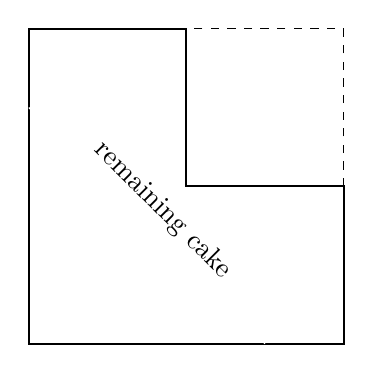
\begin{tikzpicture}
    \draw[black,thick] (0,0) -- (4,0) -- (4,2) --  (2,2) -- (2,4) -- (0,4) -- cycle;
    \draw[dashed] (4,2) -- (4,4) -- (2,4);
    \draw[white] (0,3)  -- (3,0) node [midway,sloped,above,black] {remaining cake};
    \end{tikzpicture}                
    \end{figure}
\end{enumerate}
\end{document}

\newpage
\thispagestyle{empty}
\centering
\begin{minipage}{0.8\textwidth}
    \vspace{3cm}
    Monthly Maths Circle India Challenge is a maths competition open to everyone who likes to solve mathematical problems. Every second Friday of the month, we will upload a new problem on our website. You will have three weeks to solve it and submit your answer before the deadline specified on the challenge sheet. Anyone can join, regardless of their age. We seek creative solutions that show a good understanding of various mathematical concepts. Please avoid using computer programs or excessively lengthy calculations. We will evaluate your submission based on its completeness, accuracy, and presentation quality. Remember that this contest aims to stimulate mathematical creativity; our graders' decisions are final.
\end{minipage}
\centering
\begin{minipage}{0.8\textwidth}
    \vspace{3cm}
Check \url{https://www.icts.res.in/outreach/mci} for more information
\end{minipage}
\begin{minipage}{0.8\textwidth}
    \vspace{3cm}
    \centering
    \includegraphics[scale=0.15]{mci-monthly}

    Scan to submit your entry.
\end{minipage}